
\section{Solutions to a Sphere in Fluid}
Van Lew\cite{VanLew2010}, in the study of solar thermal energy storage considered a sphere submerged in a heat-transfer fluid to show the diverging accuracy of the lumped capacitance method as the Biot number increased above unity. Van Lew introduced a method of modifying the heat transfer coefficient, referred to as the Jeffreson correction, to correct for large $\Bi$. The correction technique was further generalized by Xu, et al.\cite{Xu2012} for large Biot numbers with more generic geometries. We will show here how the same technique can be applied when nuclear heating of the solid is introduced. The solution technique is similar to the detailed process given by Van Lew\cite{VanLew2010} so some details will be omitted here.

We consider a single sphere with volumetric heat generation submerged in and thermally interacting with a fluid. The sphere will be of radius $R=d_p/2$, as shown in Fig.~\ref{fig:ParticleControlVolume}. The sphere will initially be at a uniform temperature of $T_i$. The fluid temperature will remain constant at $T_f$

\begin{figure}[ht]
	\centering
		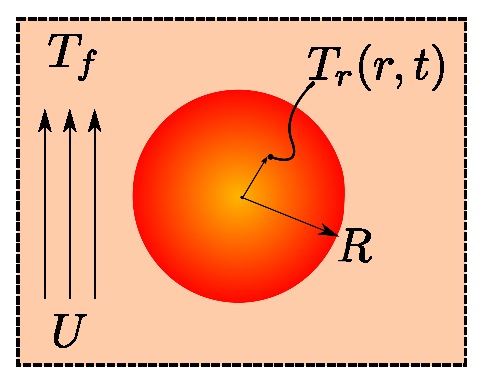
\includegraphics[width=2in]{chapters/figures/ParticleControlVolume}
	\caption[Control volume of single spherical particle in a packed bed]{CONTROL VOLUME OF A SINGLE SPHERICAL PARTICLE IN A PACKED BED}
	\label{fig:ParticleControlVolume}
\end{figure}

%~~~~~~~~~~~~~~~~~~~~~~~~~~~~~~~~~~~~~~~~~~~~~~~~~~~~~~~

\subsection{Exact Solution for Sphere}

The solution will be found for temperature in dimensionless form. We scale by the maximum temperature difference occuring at the initial state,

\begin{equation}
	\theta=\frac{T(r,t)-T_{f}}{T_{i}-T_{f}}
\end{equation}

where $T(r,t)$ is the temperature of the sphere as it varies in radius and time. The solution is given in terms of a dimensionless time (Fourier number), $\Fo = \frac{t}{R^2/\alpha}$, and non-dimensional radius $r^* = \frac{r}{R}$,

\begin{equation}
	\theta_{t.g.}=\sum_{n=1}^\infty C_n exp(-\zeta_n^2 \Fo)\frac{1}{\zeta_nr^*} sin(\zeta_n r^*)
\end{equation}

where we designate $\theta_{t.g.}$ as the dimensionless temperature specific for exact solution with thermal gradient. The coefficients are

\begin{equation}
	C_n=\frac{4\big(sin\zeta_n -\zeta_n cos\zeta_n\big)}{2\zeta_n-sin(2\zeta_n)}
\end{equation}

and the discrete values of $\zeta_n$ are positive roots of the transcendental equation

\begin{equation}\label{eq:traneqn}
	1-\zeta_ncot\zeta_n = \Bi
\end{equation}

where the first 10 roots of the transcendental equation are solved for numerically with the Newton-Raphson method of root finding. The total amount of energy removed from the sphere at time $t$ is given in the same dimensionless form as Van Lew\cite{VanLew2010}, 

\begin{equation}
	Q^*=\frac{Q}{Q_{\infty}}
\end{equation}

where $Q_{\infty}$ is the total, thermal potential energy of the sphere,

\begin{equation}
	Q_{\infty}=\rho_rC_rV(T_{i}-T_{f})
\end{equation}

The total removed energy is then

\begin{equation}
\label{eq:qexact}
	Q^*_{t.g.}=1-3\sum_{n=1}^\infty C_n exp(-\zeta_n^2 Fo)\frac{1}{\zeta_n^3} \big(sin\zeta_n-\zeta_ncos\zeta_n\big)
\end{equation}

Equation~\ref{eq:qexact} is the exact solution for the amount of heat removed from a sphere as a function of dimensionless time~$Fo$. We will use this value for a direct comparison with the lumped capacitance method.



%~~~~~~~~~~~~~~~~~~~~~~~~~~~~~~~~~~~~~~~~~~~~~~~~~~~~~~~

\subsection{Lumped Capacitance Solution for Sphere}
The dimensionless temperature curve, $\theta_{l.c.}^*$, is found from a simple balance of the change in internal energy with the convective transport of energy away from the solid.  

\begin{equation}
	hA(T_s-T_f)=-\rho_sC_sV\frac{dT}{dt} + q_g'''V
\end{equation}

With dimensionless temperature, a first order differential arises and the solution is simply:

\begin{equation}
\label{eq:thetalc}
	\theta_{l.c.}=exp\left(-\frac{hA}{\rho_s C_s V}t\right) + G
\end{equation}

where the dimensionless heat generation term is 

\begin{equation}
	G = \frac{q_g'''}{\rho_sC_s(T_{i}-T_{f})}
\end{equation}

To find the heat transfer out of a sphere with the Lumped Capacitance Method, we balance the change in the internal energy of the sphere with the quantity of heat transferred to the fluid, $E_{st} = Q_{\text{out}}$. In dimensionless form, the energy equation simplifies to the simple form of

\begin{equation}
	Q^*_{l.c.}=1-\theta^*_{l.c.}
\label{eq:qlc}
\end{equation}



\begin{figure}[ht]
	\centering
		\includegraphics[width=4in]{chapters/figures/qlcandqexact}
	\caption[Heat transfer solutions for single sphere]{HEAT TRANSFER SOLUTIONS FOUND IN TIME VIA THE LUMPED CAPACITANCE METHOD AND EXACT SOLUTION FOR SPHERE}
	\label{fig:qlcandqexact}
\end{figure}

%~~~~~~~~~~~~~~~~~~~~~~~~~~~~~~~~~~~~~~~~~~~~~~~~~~~~~~~

\subsection{Jeffreson Correction Solution}
A correlation to correct the heat transfer coefficient due to solids with large Biot number is given by Jeffreson\cite{jeffreson409}. The correction has been used to successfully account for using the lumped capacitance method with moderately sized Biot numbers. We introduce it here to the case of a sphere with Biot number greater than unity and experiencing volumetric heat generation. The Jeffreson correction for a sphere is,

\begin{equation}
	\frac{1}{h_{p}}=\frac{1+Bi/5}{h}
\end{equation}

where $h_p$ is the modified heat transfer coefficient of the particle with an internal temperature gradient.  An increase in the Biot Number (or increase of thermal gradient inside the solid) results in a decrease in the heat transfer coefficient~$h_p$.  Applying the Jeffreson Correction to Eq.~\ref{eq:thetalc} and thereby Eq.~\ref{eq:qlc} gives,

\begin{equation}
	\theta^*_{j.c.}=exp\bigg(-\frac{h_{p}A}{\rho_r C_rV}t\bigg)
\end{equation}

and

\begin{equation}
\label{eq:qjc}
	Q^*_{j.c.}=1-\theta^*_{j.c.}
\end{equation}

We now compare the total heat removed from the sphere as found from the exact solution, Eq.~\ref{eq:qexact}, the standard lumped capacitance method, Eq.~\ref{eq:qlc}, and the lumped capacitance with Jeffreson correction, Eq.~\ref{eq:qjc}.

%~~~~~~~~~~~~~~~~~~~~~~~~~~~~~~~~~~~~~~~~~~~~~~~~~~~~~~~
\subsection{Results}
Plotted in Fig.~\ref{qvstime_lc_jc_tg} is a comparison between the non-dimensional heat transfers out of the sphere as functions of time for three different methods: Lumped Capacitance, Lumped Capacitance with Jeffreson Correction, and the Exact Solution with thermal gradient. As discussed in Fig.~\ref{fig:qlcandqexact}  the curve for Lumped Capacitance Method quickly approaches $Q^*=1$. The exact solution seems to lag behind this curve. This lag appears to be well accounted for with the reduced heat transfer coefficient as given by the Jeffreson Correction.  The curve for the Jeffreson Correction method closely matches that of the model for the Temperature Gradient for all dimensionless time.  

The Jeffreson Correction method accurately models the the thermodynamics of a system with a Biot Number larger while still allowing the simplified calculation of the lumped capacitance method.

\begin{figure}[ht]
	\begin{center}
		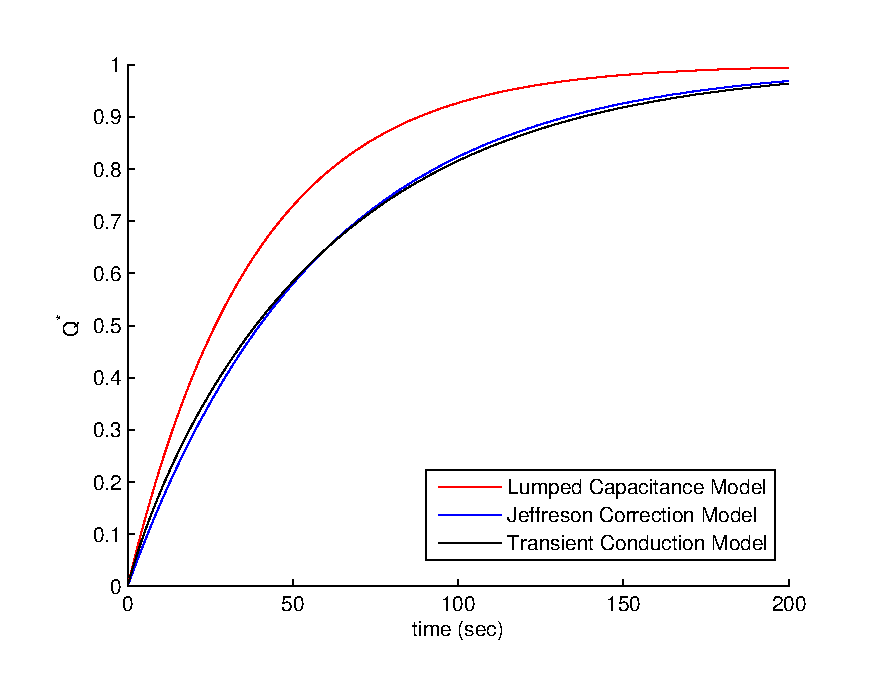
\includegraphics[width=4in]{chapters/figures/Qvstime_lc_jc_tg} 
	\end{center}
	\caption[Heat transfer solutions with correction for single sphere]{HEAT TRANSFER SOLUTIONS FOUND IN TIME VIA THE LUMPED CAPACITANCE METHOD, JEFFRESON CORRECTION, AND EXACT SOLUTION FOR SPHERE WITH $Bi=2.54$}
	\label{qvstime_lc_jc_tg} 
\end{figure}